\chapter{Controller specific implementations}
\renewcommand{\baselinestretch}{\mystretch}
\label{chap:BG}
%\setlength{\parindent}{0pt}

To setup a reference baseline for optimal performance, sequence rendering applications dedicated to specific controllers were developed. These applications take the same sequence data file, but support only the \texttt{TCPLinky} controller developed in \sref{sec:tcplinky}. These programs were implemented as simple as possible without all intermediate layers, but still use a threading structure same as the original Vixen application.

\section{Qt2 based implementation}

A GUI application dedicated to the \texttt{TCPLinky} was developed using C++ as an optional user-friendly alternative implementation showcase. This application was developed specific to the Noah NP1380 platform listed in \sref{sec:systems}. This device is a handheld embedded device based on a 10 years old SoC chip, originally designed for educational use. \fref{fig:noah_main} shows the main interface of this device. Fortunately, this devices uses Linux system and Qt2 as GUI. Therefore, it is possible to test Vixen application on this low-end platform.

\begin{figure*}[t]
  \centering
  \subfloat[Main GUI]{\includegraphics[width=0.45\textwidth]{Figs/noah.png}%
  \label{fig:noah_main}}
  \hfil
  \subfloat[Controller application]{\includegraphics[width=0.45\textwidth]{Figs/vixen_noah.png}%
  \label{fig:vixen_noah}}
  \caption{Screenshot of Noah NP1380 device}
  \label{fig:noah}
\end{figure*}

\fref{fig:vixen_noah} shows a screenshot of the dedicated application. The method of performance profiling through statistic files in proc file system was also tested. These smaller progress bars at the lower half of the application shows percentages of CPU time spent on different tasks, such as user space applications, kernel mode and interrupt handling. Most of the time only less than $50 \%$ CPU time was used for this controller application, indicates even this low-end device is capable of handling thousands of lighting channels.

\section{Minimal C\# implementation}

Another minimal implementation was developed using C\#, named \texttt{VixenLinky}. Source code for controller output was ported directly from the original Vixen application. All intermediate layers and DLL loading were excluded from this implementation. With this program, the best possible performance on each platform can be measured as a reference.

The overall performance of optimised Vixen may be limited by two different factors, sequence loading performance and controller update speed. Therefore, options to unlimit the update interval of both sequence loading and controller update were added separately.

\fref{fig:vixenlinky_noah} shows an example of performance data gathered on the Noah NP1380 platform through \texttt{VixenLinky} using one of real-world lighting sequences. The refresh rates of both playback and controller are very stable around 50 fps. The CPU usage peaks at $60.0 \%$ while most of the time distributed around $20.0 \%$ and $30.0 \%$ (first and third quartiles).

\begin{figure}[!t]
  \centering
  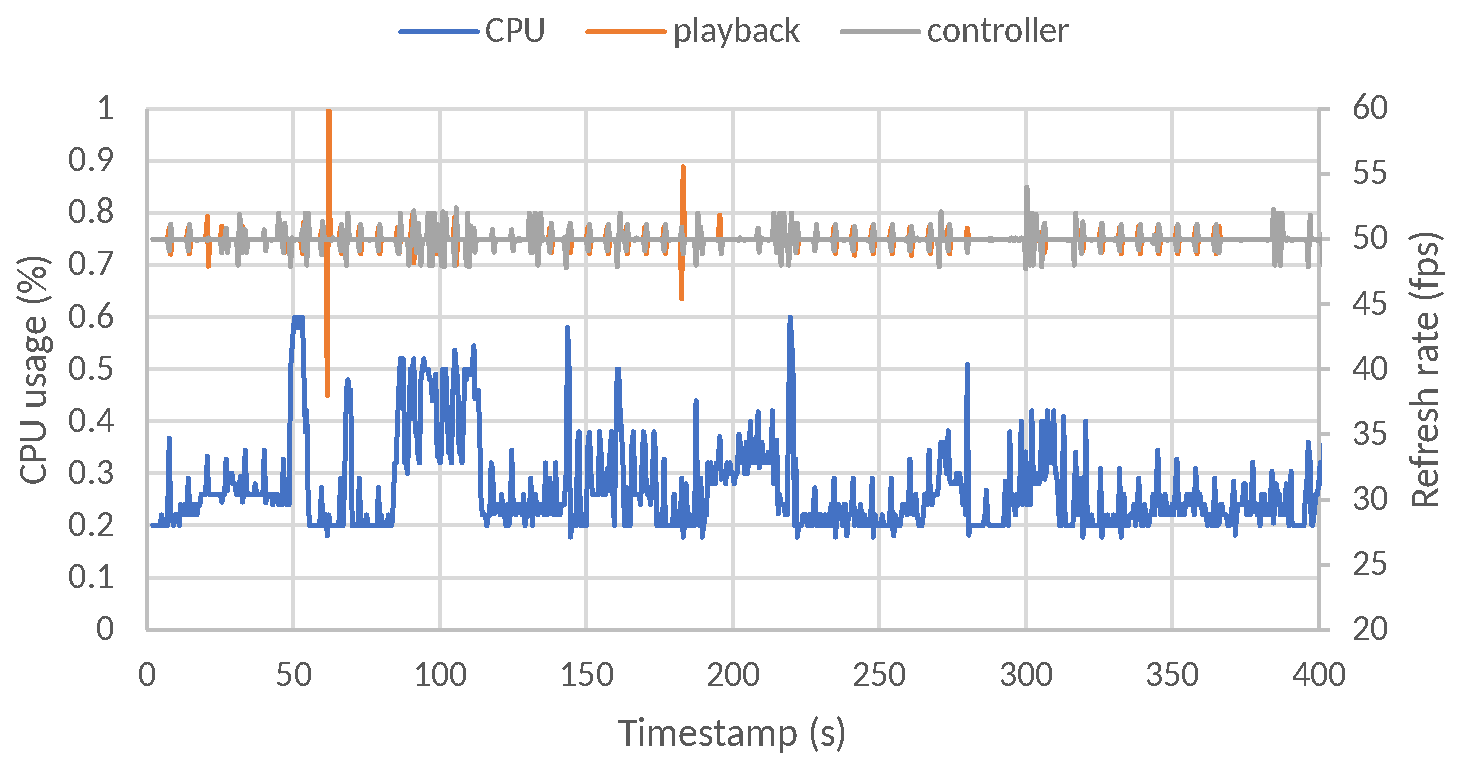
\includegraphics[width=0.8\columnwidth]{Figs/vixenlinky_noah.eps}
  \caption{Performance of \texttt{VixenLinky} on Noah NP1380}
  \label{fig:vixenlinky_noah}
\end{figure}
